110. Алёша отправил по почте 2 письма Олегу. Изначально у Алёши было 6 марок, которые стоили 20 рублей, 24 рубля, 28 рублей, 32 рубля, 36 рублей и 40 рублей. После отправки у Алёши осталась одна марка. Какая марка могла остаться, если письма стоили одинаково?

ewpage

oindent111. Из одинаковых кубиков склеена фигура. Её сфотографировали спереди, сверху и справа. Каким может быть максимальное количество кубиков в этой фигуре?
\begin{center}
\begin{figure}[ht!]
\center{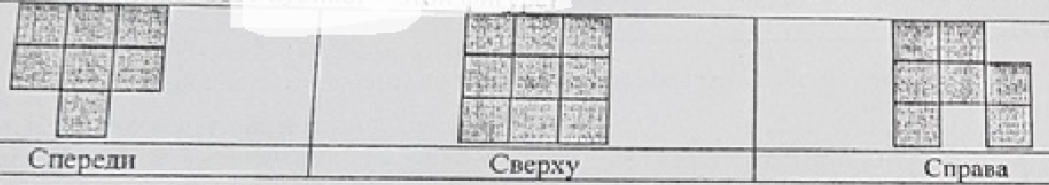
\includegraphics[scale=0.35]{19.png}}
\end{figure}
\end{center}
